\documentclass[convert={density=300,size=1080x800,outext=.png}]{standalone}
\usepackage{tikz}
\usepackage{float}
\usetikzlibrary{shapes,arrows,positioning,calc, fit, backgrounds, graphs, shadows}
\usepackage{listings}

\newcommand{\class}[1]{{\small\textsf{#1}}}

% to convert to png
% pdflatex -shell-escape pipeline_diagram.tex

\begin{document}
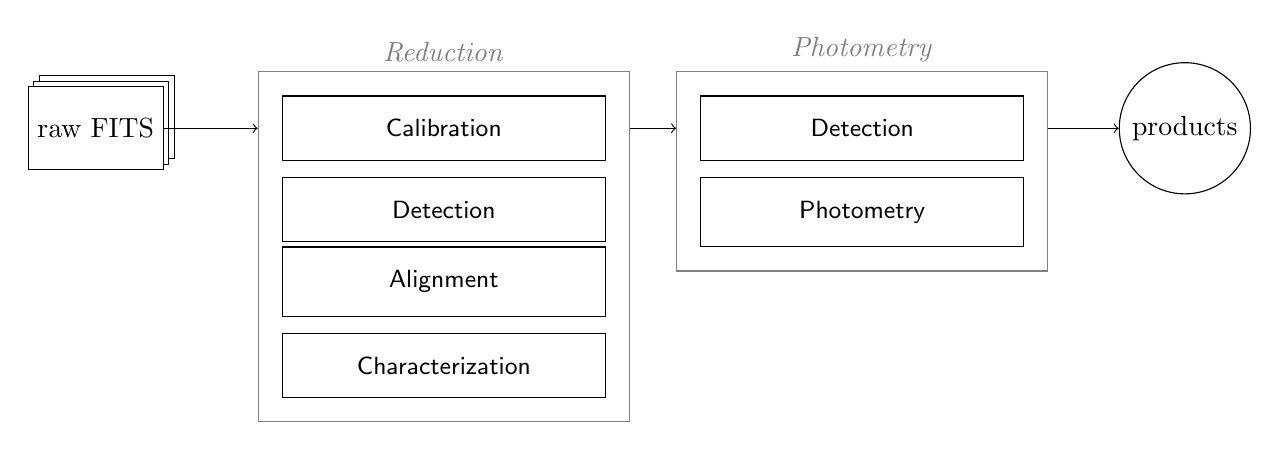
\begin{tikzpicture}[
    inblock/.style = {rectangle, draw, align=center, text width=3.5cm,fill=white, inner xsep=3mm, inner ysep=3mm},
    outblock/.style = {rectangle, draw, inner xsep=3mm, inner ysep=3mm, color=black!50},
    multipledoc/.style={draw, minimum height=3em, minimum width=3em, fill=white, double copy shadow={shadow xshift=2pt, shadow yshift=2pt, draw}}, 
    singledoc/.style={circle, draw, minimum height=3em, minimum width=3em, fill=white},
    ]

        % Nodes
        \node[inblock] (calib) {\class{Calibration}};
        \node[inblock, below=2mm of calib] (detect0) {\class{Detection}};
        \node[inblock, below=0.5mm of detect0] (align) {\class{Alignment}};
        \node[inblock, below=2mm of align] (char) {\class{Characterization}};
        \node[fit=(calib) (align) (char), outblock, label=above:\color{gray}\textit{Reduction}] (reduction) {};
        %
        \node[multipledoc, left=15mm of calib](input) {raw FITS};
        %
        \node[inblock, right=12mm of calib] (detect) {\class{Detection}};
        \node[inblock, below=2mm of detect] (phot) {\class{Photometry}};
        \node[fit=(detect) (phot), outblock, label=above:\color{gray}\textit{Photometry}] (photometry) {};
        %
        \node[singledoc, right=12mm of detect](output) {products};

        % Draw
        \draw [->] (input) -- (input-|reduction.west);
        \draw [->] (calib-|reduction.east) -- (calib-|photometry.west);
        \draw [->] (detect-|photometry.east) -- (output);
    \end{tikzpicture}

\end{document}